\documentclass[aspectratio=169]{beamer}
\usepackage[utf8]{inputenc}
\usepackage[T1]{fontenc}
\usepackage{lmodern}
\usepackage{xcolor}
\usepackage[portuguese]{babel}
\usepackage{amsmath}
\usepackage{booktabs}
\usepackage{tcolorbox}
\tcbuselibrary{skins,breakable}

\definecolor{BgCream}{HTML}{FAF8F5}
\definecolor{TextEspresso}{HTML}{4A4238}
\definecolor{NudeTaupe}{HTML}{BFAFA6}
\definecolor{SoftBlush}{HTML}{D9C5B2}
\definecolor{SageMuted}{HTML}{7E8F7C}
\definecolor{ClayWarn}{HTML}{B5795C}

\setbeamertemplate{navigation symbols}{}
\setbeamercolor{background canvas}{bg=BgCream}
\setbeamercolor{normal text}{fg=TextEspresso}
\setbeamercolor{structure}{fg=TextEspresso}

\setbeamertemplate{itemize item}{\color{NudeTaupe}\textendash}
\setbeamertemplate{itemize subitem}{\color{NudeTaupe}\(\circ\)}

\setbeamerfont{title}{size=\huge, series=\bfseries}
\setbeamerfont{frametitle}{size=\Large, series=\bfseries}

\setbeamertemplate{title page}{
  \vspace*{1.5cm}
  \begin{center}
    \usebeamerfont{title}\textcolor{TextEspresso}{\inserttitle}\par
    \vspace{0.35cm}
    {\large\textcolor{NudeTaupe}{\insertsubtitle}}\par
    \vspace{0.6cm}
    {\color{NudeTaupe}\rule{2.5cm}{0.5pt}}\par
    \vspace{0.8cm}
    \usebeamerfont{author}\textcolor{TextEspresso}{\insertauthor}\par
    \vspace{0.3cm}
    \usebeamerfont{institute}\small\textcolor{NudeTaupe}{\insertinstitute \quad|\quad \insertdate}
  \end{center}
}

\setbeamertemplate{frametitle}{
  \vspace*{0.8cm}
  \usebeamerfont{frametitle}\insertframetitle\par
  \vspace*{-0.1cm}
  {\color{NudeTaupe}\rule{1.5cm}{0.5pt}}
  \vspace*{0.2cm}
}

\newenvironment{ideiachave}{
  \vspace{0.5cm}
  \begin{center}
  \color{TextEspresso}
  \itshape\Large
}{
  \end{center}
  \vspace{0.5cm}
}

\newtcolorbox{pergunta}[1]{
  colback=SoftBlush!30, colframe=NudeTaupe, boxrule=0.6pt, arc=3pt,
  left=8pt, right=8pt, top=6pt, bottom=6pt,
  title={\bfseries #1}, coltitle=TextEspresso, colbacktitle=SoftBlush!60,
  fonttitle=\bfseries, fontupper=\normalsize\color{TextEspresso}
}

\newtcolorbox{resposta}[1]{
  colback=SageMuted!12, colframe=SageMuted, boxrule=0.6pt, arc=3pt,
  left=8pt, right=8pt, top=6pt, bottom=6pt,
  title={\bfseries #1}, coltitle=white, colbacktitle=SageMuted,
  fonttitle=\bfseries, fontupper=\normalsize\color{TextEspresso}
}

\usepackage{csquotes}

\title{Arquitetura de Datacenters e Modelos de Operação}
\subtitle{Infraestruturas de Computação na Nuvem, Aula 02}
\author{Catarina Silva}
\institute{ESTGA, Universidade de Aveiro}
\date{2026}

\begin{document}

\begin{frame}[plain]
  \titlepage
\end{frame}

\begin{frame}
\frametitle{Agenda \textcolor{NudeTaupe}{\small(1/3)}}
\begin{itemize}
    \setlength\itemsep{0.4cm}
    \item Definição e subsistemas constituintes de um datacenter.
    \item Domínios de falha e pontos únicos de falha.
    \item Níveis de redundância: $N$, $N+1$, $2N$.
    \item Classificação do Uptime Institute e normas alternativas.
\end{itemize}
\end{frame}

\begin{frame}
\frametitle{Agenda \textcolor{NudeTaupe}{\small(2/3)}}
\begin{itemize}
    \setlength\itemsep{0.4cm}
    \item Topologias de rede: hierárquica de três camadas e leaf-spine.
    \item Padrões de tráfego este-oeste e norte-sul.
    \item Razão de sobre-subscrição e dimensionamento de uplinks.
\end{itemize}
\end{frame}

\begin{frame}
\frametitle{Agenda \textcolor{NudeTaupe}{\small(3/3)}}
\begin{itemize}
    \setlength\itemsep{0.4cm}
    \item Quantificação da disponibilidade: MTBF, MTTR e classes de serviço.
    \item Modelos de fiabilidade em série e em paralelo.
    \item Estrutura formal de um acordo de nível de serviço.
    \item Modelos de operação, distribuição geográfica e eficiência energética.
\end{itemize}
\end{frame}

\begin{frame}
\frametitle{Definição de Datacenter}
\begin{itemize}
    \setlength\itemsep{0.4cm}
    \item Um \textbf{datacenter} é uma instalação destinada a alojar sistemas de computação e respetiva infraestrutura de suporte, dimensionada para operação contínua.
    \item A instalação compreende quatro subsistemas interdependentes: \textbf{distribuição de energia}, \textbf{controlo térmico}, \textbf{conectividade de rede} e \textbf{espaço físico} com os respetivos controlos de acesso.
    \item Os subsistemas encontram-se em dependência mútua: a indisponibilidade de qualquer um deles compromete a operação do conjunto.
    \item A presente aula analisa a organização destes subsistemas, os critérios normativos que os classificam e os modelos sob os quais são operados.
\end{itemize}
\end{frame}

\begin{frame}
\frametitle{Subsistemas de uma Instalação}
\vfill
\begin{center}
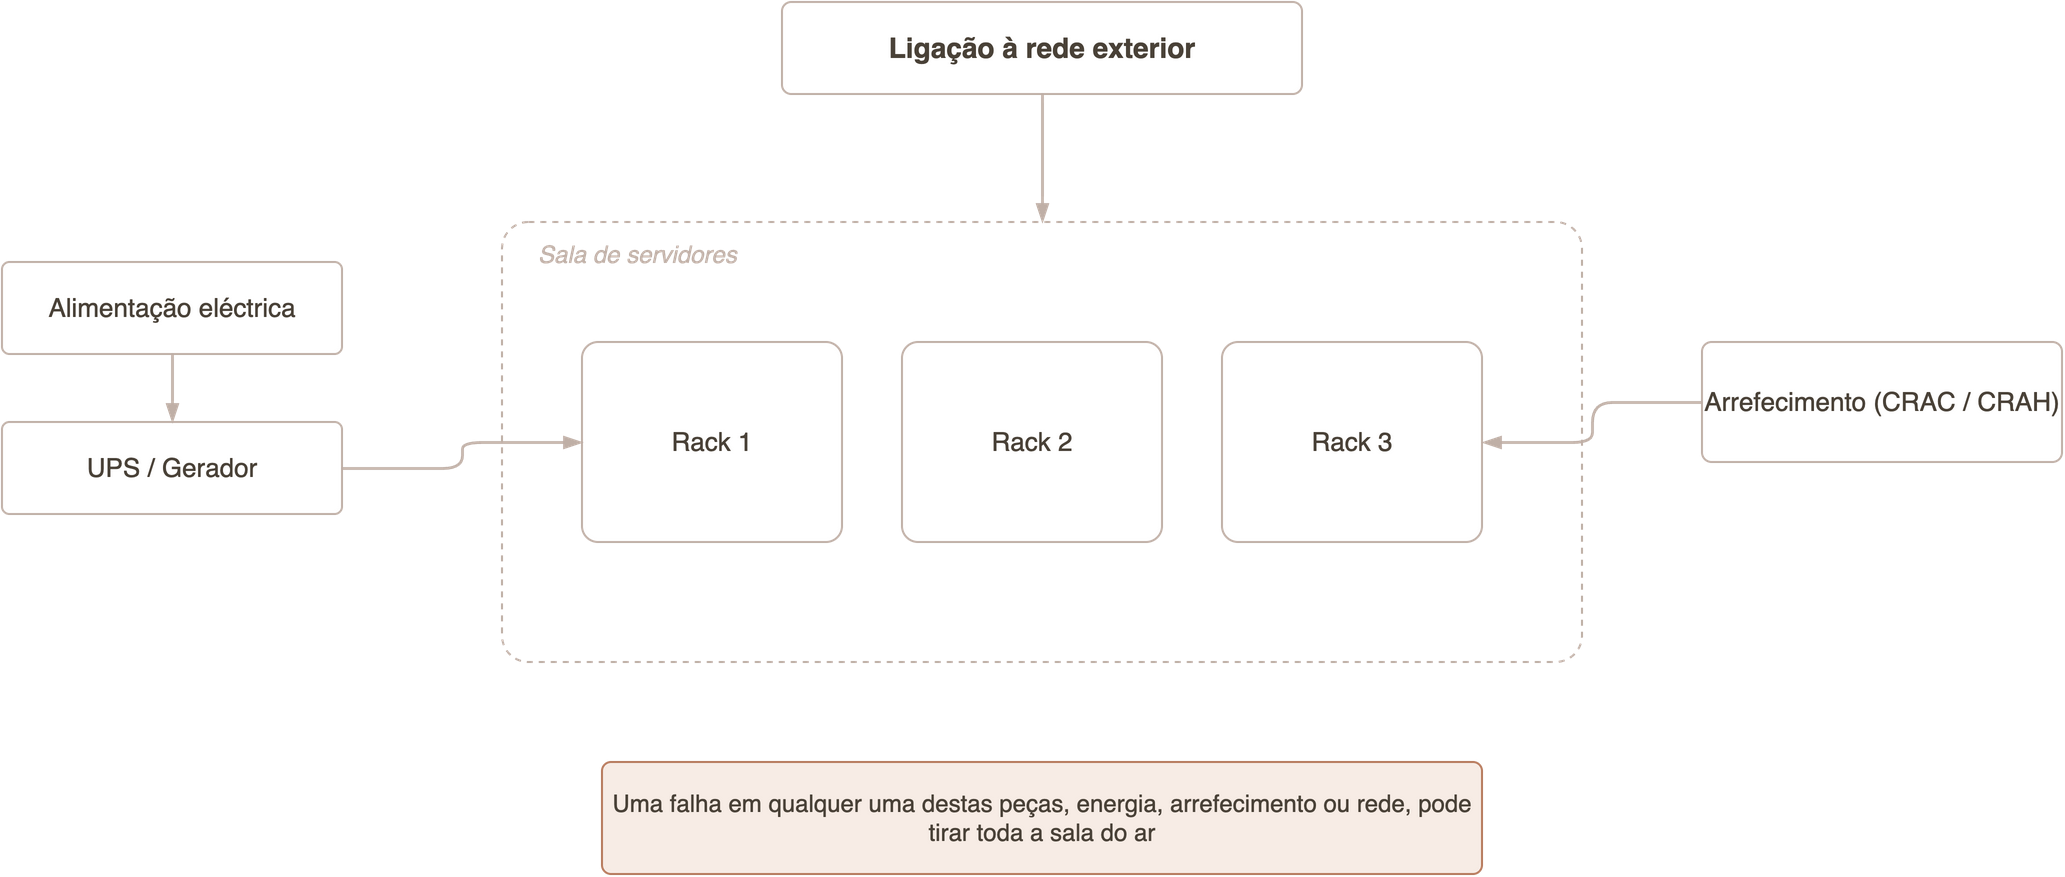
\includegraphics[width=0.95\textwidth,height=0.72\textheight,keepaspectratio]{../Diagramas/a02-anatomia-datacenter.png}
\end{center}
\vfill
\end{frame}

\begin{frame}
\frametitle{Domínios de Falha}
\begin{itemize}
    \setlength\itemsep{0.4cm}
    \item Designa-se por \textbf{domínio de falha} o conjunto de componentes afetados pela falha de um elemento comum de que todos dependem.
    \item Exemplos por subsistema: um quadro de distribuição elétrica, uma unidade de arrefecimento, um comutador de topo de bastidor, um troço de fibra óptica.
    \item Um componente cuja falha determina a indisponibilidade do sistema completo constitui um \textbf{ponto único de falha} (\emph{single point of failure}).
    \item A análise de arquitetura não se ocupa da possibilidade de falha, que se assume certa, mas da sua \emph{propagação}: que fração do sistema é afetada e por que via.
\end{itemize}
\end{frame}

\begin{frame}
\frametitle{Pergunta 1}
\begin{pergunta}{Propagação de uma falha elétrica}
Considere-se uma instalação com via única de alimentação, sem UPS nem grupo gerador. Durante uma manutenção, essa via é inadvertidamente interrompida. Qual o efeito sobre o serviço?
\begin{itemize}
    \item[A)] Nulo. As fontes dos servidores asseguram autonomia até ao restabelecimento.
    \item[B)] Indisponibilidade total e imediata de todos os sistemas alojados, até ao restabelecimento da alimentação.
    \item[C)] Comutação automática para a alimentação de uma instalação adjacente.
    \item[D)] Paragem apenas do armazenamento, mantendo-se o processamento.
\end{itemize}
\end{pergunta}
\end{frame}

\begin{frame}
\frametitle{Resposta 1}
\begin{resposta}{Opção correta: B}
Na ausência de UPS e de grupo gerador não existe via alternativa de alimentação: a via única constitui um ponto único de falha cujo domínio abrange a totalidade da instalação. As fontes de alimentação dos servidores asseguram estabilização na ordem dos milissegundos, insuficiente para cobrir uma interrupção prolongada. A configuração descrita corresponde ao nível mais baixo da classificação que se apresenta em seguida.
\end{resposta}
\end{frame}

\begin{frame}
\frametitle{Níveis de Redundância}
\begin{itemize}
    \setlength\itemsep{0.4cm}
    \item Sendo a falha inevitável, o critério de projeto relevante é o número de vias alternativas disponíveis antes da interrupção do serviço.
    \item \textbf{$N$}: capacidade estritamente necessária para sustentar a carga nominal, sem margem.
    \item \textbf{$N+1$}: acresce uma unidade de reserva ao conjunto necessário. Tolera a indisponibilidade de um componente, mantendo-se a via de distribuição única.
    \item \textbf{$2N$}: duplicação integral do subsistema, incluindo as vias de distribuição. Tolera a perda de metade da instalação sem degradação do serviço.
    \item Variante intermédia frequente: \textbf{$2(N+1)$}, aplicada quando se exige manutenção concorrente sobre uma via já redundante.
\end{itemize}
\end{frame}

\begin{frame}
\frametitle{Classificação Uptime Institute \textcolor{NudeTaupe}{\small(1/2)}}
\begin{itemize}
    \setlength\itemsep{0.4cm}
    \item O Uptime Institute classifica a \emph{topologia} da infraestrutura em quatro níveis (Tiers), de I a IV, em função da redundância e da tolerância a falhas.
    \item A classificação incide sobre a organização dos subsistemas, e não sobre o desempenho, a dimensão ou a qualidade do equipamento instalado.
    \item \textbf{Tier I}: infraestrutura de capacidade básica, sem redundância. Qualquer intervenção de manutenção ou avaria implica interrupção do serviço.
    \item \textbf{Tier II}: componentes de capacidade redundantes ($N+1$), mantendo-se uma via única de distribuição, que permanece como ponto único de falha.
\end{itemize}
\end{frame}

\begin{frame}
\frametitle{Classificação Uptime Institute \textcolor{NudeTaupe}{\small(2/2)}}
\begin{itemize}
    \setlength\itemsep{0.4cm}
    \item \textbf{Tier III}: múltiplas vias de distribuição independentes, das quais uma se encontra ativa. Admite \emph{manutenção concorrente}, isto é, a intervenção sobre qualquer componente sem interrupção do serviço.
    \item \textbf{Tier IV}: tolerância a falhas com redundância $2N$ em todos os componentes críticos e compartimentação física entre vias. Uma falha única não produz efeito observável no serviço.
    \item Critério determinante: o nível atribuído corresponde ao do \emph{subsistema menos redundante}, e não à média dos subsistemas.
\end{itemize}
\end{frame}

\begin{frame}
\frametitle{Pergunta 2}
\begin{pergunta}{Atribuição de nível}
Uma instalação dispõe de duas vias de alimentação elétrica independentes, cada uma com grupo gerador próprio, e de duas vias de rede distintas. O subsistema de arrefecimento é constituído por uma única unidade, sem reserva. Que nível lhe é atribuível?
\begin{itemize}
    \item[A)] Tier IV, por dispor de dupla via de energia e de rede.
    \item[B)] Tier III, por dispor de vias independentes em parte dos subsistemas.
    \item[C)] Nível limitado pelo subsistema de arrefecimento, não sendo classificável como Tier III nem como Tier IV.
    \item[D)] Tier II, por dispor de pelo menos uma unidade de reserva.
\end{itemize}
\end{pergunta}
\end{frame}

\begin{frame}
\frametitle{Resposta 2}
\begin{resposta}{Opção correta: C}
A classificação incide sobre o conjunto dos subsistemas críticos. A unidade de arrefecimento sem reserva constitui um ponto único de falha cujo domínio abrange a sala completa: em caso de avaria, a temperatura excede os limites de operação e os sistemas desligam-se por proteção térmica, independentemente do estado da alimentação e da rede. O nível atribuível é, por conseguinte, determinado pelo subsistema menos redundante.
\end{resposta}
\end{frame}

\begin{frame}
\frametitle{Normas de Classificação}
\begin{itemize}
    \setlength\itemsep{0.35cm}
    \item A classificação do Uptime Institute é a de utilização mais generalizada, coexistindo com normas de âmbito distinto.
    \item \textbf{ANSI/TIA-942}: norma norte-americana de infraestrutura de telecomunicações, que define os níveis \emph{Rated-1} a \emph{Rated-4} e abrange adicionalmente cablagem estruturada, disposição do espaço e proteção contra incêndio.
    \item \textbf{EN 50600}: série normativa europeia, com classes de disponibilidade de 1 a 4, integrando requisitos de eficiência energética e de segurança física.
    \item As escalas são análogas em princípio mas não estabelecem equivalência formal entre si; a norma aplicada deve ser explicitada em qualquer caracterização.
\end{itemize}
\end{frame}

\begin{frame}
\frametitle{Topologia Hierárquica de Três Camadas}
\begin{itemize}
    \setlength\itemsep{0.4cm}
    \item Organização clássica em três camadas: \textbf{core}, \textbf{aggregation} e \textbf{access}.
    \item A camada \emph{core} assegura a ligação ao exterior e o encaminhamento entre blocos; a camada \emph{aggregation} concentra o tráfego e delimita domínios de difusão; a camada \emph{access} liga os servidores.
    \item O encaminhamento entre servidores alojados em bastidores distintos exige a travessia ascendente e descendente da hierarquia, com acréscimo de latência proporcional ao número de saltos.
    \item A latência entre dois servidores depende, assim, da respetiva localização física, o que compromete a previsibilidade do desempenho.
\end{itemize}
\end{frame}

\begin{frame}
\frametitle{Topologia Leaf-Spine}
\begin{itemize}
    \setlength\itemsep{0.4cm}
    \item Topologia derivada das redes de Clos: cada comutador \emph{leaf} estabelece ligação a todos os comutadores \emph{spine}, não existindo adjacências diretas entre leafs nem entre spines.
    \item O percurso entre quaisquer dois servidores ligados a leafs distintos compreende exatamente dois saltos, independentemente da localização física.
    \item A multiplicidade de percursos equivalentes permite distribuição de carga por ECMP (\emph{Equal-Cost Multi-Path}), com agregação da largura de banda disponível.
    \item A capacidade agregada escala pela adição de spines; a densidade de portas de cada spine determina o número máximo de leafs suportados.
\end{itemize}
\end{frame}

\begin{frame}
\frametitle{Comparação das Topologias}
\vfill
\begin{center}
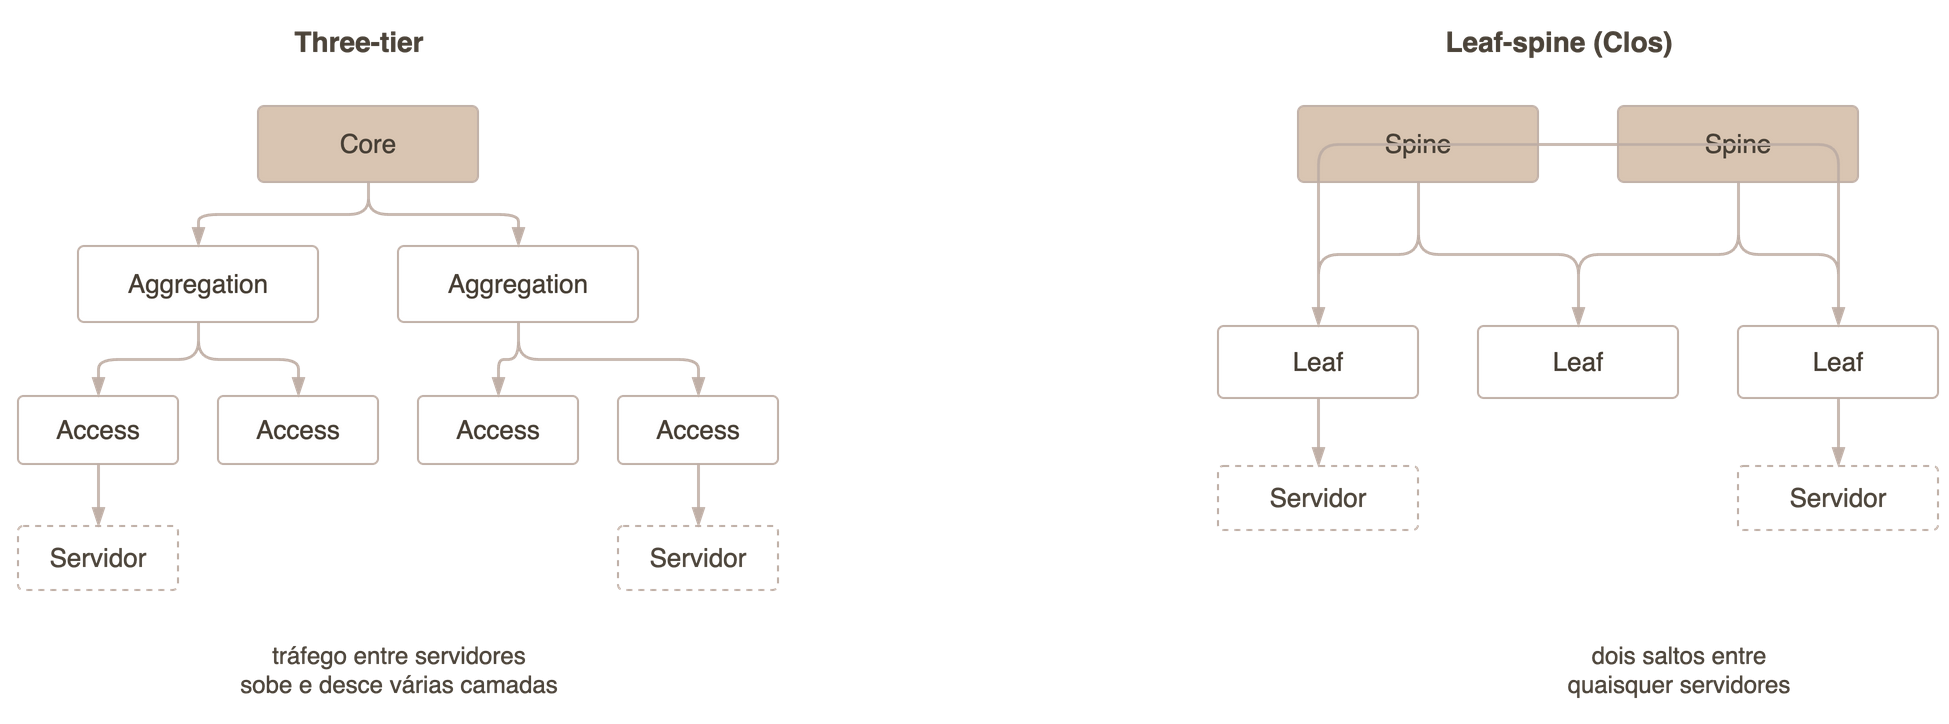
\includegraphics[width=0.97\textwidth,height=0.70\textheight,keepaspectratio]{../Diagramas/a02-topologias.png}
\end{center}
\vfill
\end{frame}

\begin{frame}
\frametitle{Padrões de Tráfego}
\begin{itemize}
    \setlength\itemsep{0.4cm}
    \item \textbf{Tráfego norte-sul}: atravessa a fronteira da instalação, entre clientes externos e os sistemas alojados.
    \item \textbf{Tráfego este-oeste}: circula entre sistemas internos, resultante de invocações entre componentes de uma mesma aplicação.
    \item A decomposição de aplicações monolíticas em serviços distribuídos inverteu a proporção histórica entre os dois padrões: um único pedido externo pode originar dezenas de invocações internas.
    \item A topologia leaf-spine responde a este padrão ao uniformizar a distância entre quaisquer dois pontos internos da rede.
\end{itemize}
\end{frame}

\begin{frame}
\frametitle{Razão de Sobre-subscrição}
\begin{itemize}
    \setlength\itemsep{0.35cm}
    \item Define-se \textbf{razão de sobre-subscrição} como o quociente entre a largura de banda agregada dos portos descendentes e a largura de banda agregada dos portos ascendentes de um comutador.
    \item Exemplo: um leaf com 48 portos de 10\,Gbit/s para servidores e 4 portos de 40\,Gbit/s para spines apresenta
    \[
      \text{razão} \;=\; \frac{48 \times 10}{4 \times 40} \;=\; \frac{480}{160} \;=\; 3{:}1 .
    \]
    \item Uma razão de $1{:}1$ designa-se por \emph{non-blocking}: qualquer padrão de tráfego é suportado sem contenção, ao custo de capacidade de uplink adicional.
    \item O valor admissível decorre do padrão de tráfego previsto; cargas com tráfego este-oeste intenso exigem razões mais próximas da unidade.
\end{itemize}
\end{frame}

\begin{frame}
\frametitle{Caso de Análise: Seleção de Topologia}
\begin{itemize}
    \setlength\itemsep{0.35cm}
    \item Considere-se uma plataforma de distribuição de vídeo decomposta em cerca de 200 serviços, entre os quais autenticação, catálogo, recomendação e faturação.
    \item O volume de invocações entre serviços excede substancialmente o volume de tráfego proveniente de clientes externos, sem que se identifique um padrão estável de comunicação entre pares.
    \item Encontra-se em fase de projeto a rede da instalação destinada a alojar a plataforma.
\end{itemize}
\vspace{0.2cm}
{\small\color{NudeTaupe}\textbf{Discussão (2 minutos):} que topologia se justifica, e que consequências decorreriam da alternativa?}
\end{frame}

\begin{frame}
\frametitle{Pergunta 3}
\begin{pergunta}{Decisão de projeto}
Para a plataforma descrita, com predominância de tráfego este-oeste e padrão de comunicação entre pares não determinístico, que topologia se justifica?
\begin{itemize}
    \item[A)] Hierárquica de três camadas, por maturidade e generalização de uso.
    \item[B)] Leaf-spine, por assegurar distância constante de dois saltos entre quaisquer servidores e admitir agregação de percursos por ECMP.
    \item[C)] Indiferente, dado que a topologia não condiciona o desempenho de aplicações distribuídas.
    \item[D)] Hierárquica de três camadas, dado que a camada \emph{core} assegura o encaminhamento entre bastidores.
\end{itemize}
\end{pergunta}
\end{frame}

\begin{frame}
\frametitle{Resposta 3}
\begin{resposta}{Opção correta: B}
Não sendo determinístico o padrão de comunicação, qualquer par de serviços pode requerer comunicação em qualquer instante. Na topologia hierárquica, a latência depende da localização relativa dos servidores, introduzindo variabilidade não controlável no tempo de resposta agregado de um pedido que encadeia dezenas de invocações. A topologia leaf-spine uniformiza essa distância e, por ECMP, distribui o tráfego pelos percursos equivalentes disponíveis.
\end{resposta}
\end{frame}

\begin{frame}
\frametitle{Quantificação da Disponibilidade}
\begin{itemize}
    \setlength\itemsep{0.35cm}
    \item Define-se \textbf{disponibilidade} $A$ como a fração do tempo em que o sistema presta serviço conforme a especificação:
    \[
      A \;=\; \frac{T_{\text{operacional}}}{T_{\text{operacional}} + T_{\text{indisponível}}} .
    \]
    \item Em regime estacionário, exprime-se em função dos tempos médios característicos:
    \[
      A \;=\; \frac{\mathrm{MTBF}}{\mathrm{MTBF} + \mathrm{MTTR}} .
    \]
    \item \textbf{MTBF} (\emph{Mean Time Between Failures}): tempo médio entre falhas consecutivas. \textbf{MTTR} (\emph{Mean Time To Repair}): tempo médio de restabelecimento do serviço.
    \item A disponibilidade admite ainda interpretação probabilística: $A$ é a probabilidade de o sistema se encontrar operacional num instante arbitrário, o que fundamenta a composição de componentes apresentada adiante.
\end{itemize}
\end{frame}

\begin{frame}
\frametitle{Implicações de MTBF e MTTR}
\begin{itemize}
    \setlength\itemsep{0.35cm}
    \item A expressão $A = \mathrm{MTBF}/(\mathrm{MTBF}+\mathrm{MTTR})$ admite duas estratégias distintas de melhoria da disponibilidade.
    \item \textbf{Aumentar o MTBF}: atuar sobre a frequência das falhas, por seleção de componentes, redundância e controlo de condições de operação.
    \item \textbf{Reduzir o MTTR}: atuar sobre a duração da interrupção, por deteção automática, diagnóstico assistido, peças de substituição em reserva e procedimentos de recuperação ensaiados.
    \item Em sistemas distribuídos, a redução do MTTR apresenta frequentemente melhor relação custo-benefício do que o aumento do MTBF, por não exigir substituição de hardware.
\end{itemize}
\end{frame}

\begin{frame}
\frametitle{Classes de Disponibilidade e Indisponibilidade Admissível}
\vspace{0.2cm}
\begin{center}
\begin{tabular}{@{}lrr@{}}
\toprule
\textbf{Disponibilidade} & \textbf{Por ano} & \textbf{Por mês (30 d)} \\
\midrule
99{,}0\,\%    & 87\,h 36\,min   & 7\,h 12\,min  \\
99{,}5\,\%    & 43\,h 48\,min   & 3\,h 36\,min  \\
99{,}9\,\%    & 8\,h 46\,min    & 43\,min 12\,s \\
99{,}99\,\%   & 52\,min 34\,s   & 4\,min 19\,s  \\
99{,}999\,\%  & 5\,min 15\,s    & 26\,s         \\
\bottomrule
\end{tabular}
\end{center}
\vspace{0.3cm}
\begin{itemize}
    \setlength\itemsep{0.25cm}
    \item Cada ordem de grandeza adicional reduz por um fator de dez a indisponibilidade admissível, exigindo alteração qualitativa da arquitetura.
    \item A partir de 99{,}99\,\%, o orçamento anual não comporta intervenção manual: a deteção e a recuperação têm de ser automáticas.
\end{itemize}
\end{frame}

\begin{frame}
\frametitle{Composição em Série}
\begin{itemize}
    \setlength\itemsep{0.35cm}
    \item Componentes dizem-se em \textbf{série} quando a totalidade é necessária ao funcionamento do sistema. Admitindo independência estatística das falhas:
    \[
      A_{\text{série}} \;=\; \prod_{i=1}^{n} A_i .
    \]
    \item Sendo $A_i \le 1$ para todo o $i$, verifica-se $A_{\text{série}} \le \min_i A_i$: a composição em série não excede a disponibilidade do componente menos disponível.
    \item Daqui decorre que o acréscimo de dependências em série degrada necessariamente a disponibilidade do conjunto, ainda que cada dependência seja individualmente fiável.
\end{itemize}
\end{frame}

\begin{frame}
\frametitle{Composição em Paralelo}
\begin{itemize}
    \setlength\itemsep{0.35cm}
    \item Componentes dizem-se em \textbf{paralelo} quando é suficiente que um se mantenha operacional. A indisponibilidade do conjunto exige a falha simultânea de todos:
    \[
      A_{\text{paralelo}} \;=\; 1 - \prod_{i=1}^{n} (1 - A_i) .
    \]
    \item Verifica-se $A_{\text{paralelo}} \ge \max_i A_i$: a redundância eleva a disponibilidade acima da de qualquer componente individual.
    \item A validade da expressão depende da hipótese de \textbf{independência das falhas}. Componentes que partilham alimentação, via de rede ou versão de software apresentam correlação, e a disponibilidade efetiva é inferior à calculada.
\end{itemize}
\end{frame}

\begin{frame}
\frametitle{Representação dos Dois Modelos}
\vfill
\begin{center}
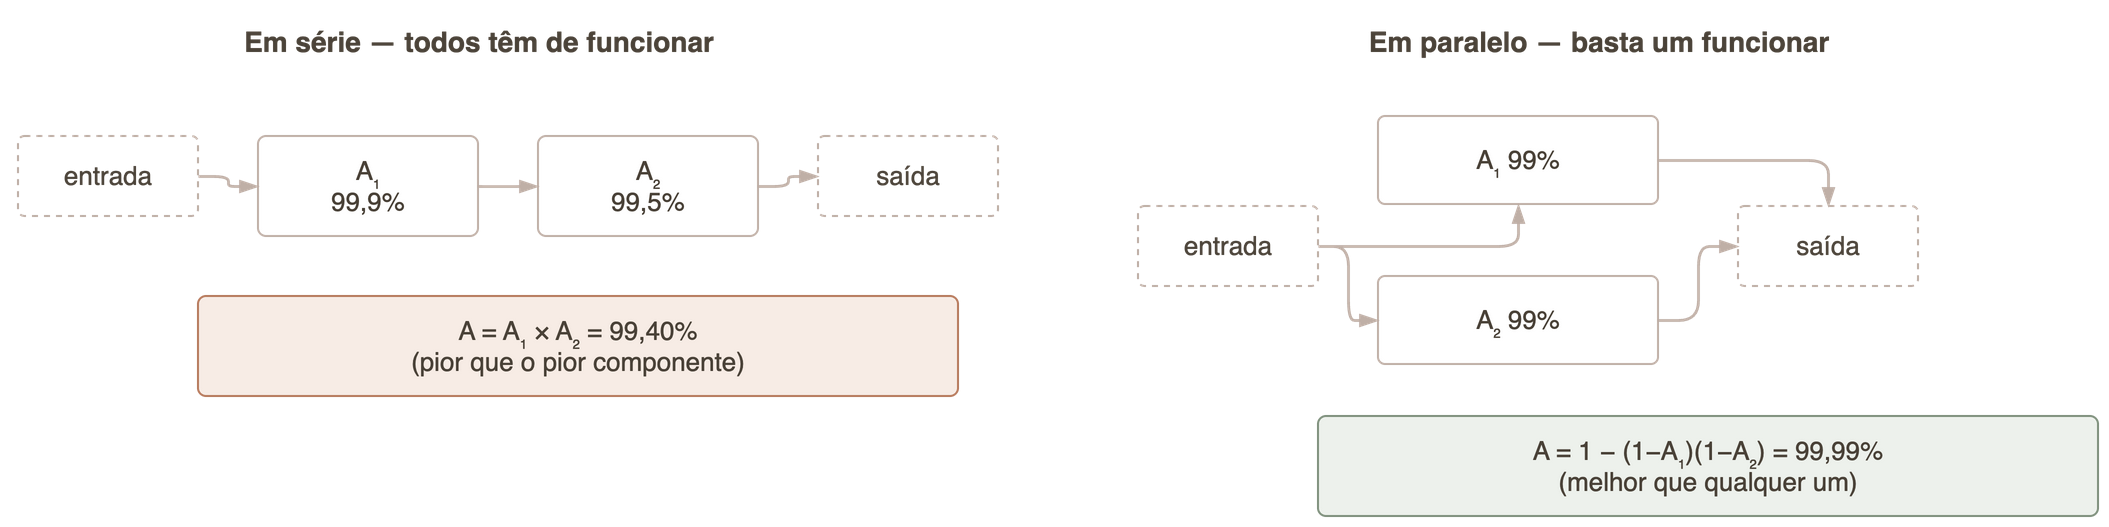
\includegraphics[width=0.97\textwidth,height=0.70\textheight,keepaspectratio]{../Diagramas/a02-serie-paralelo.png}
\end{center}
\vfill
\end{frame}

\begin{frame}
\frametitle{Exemplo: Composição em Série}
\begin{itemize}
    \setlength\itemsep{0.35cm}
    \item Um serviço depende de um encaminhador com $A_1 = 0{,}9995$ e de uma instância de base de dados sem réplica com $A_2 = 0{,}995$, ambos necessários ao funcionamento.
    \item Aplicando a expressão da composição em série:
    \[
      A \;=\; 0{,}9995 \times 0{,}995 \;=\; 0{,}99450 \;\approx\; 99{,}45\,\% .
    \]
    \item A indisponibilidade anual correspondente é de aproximadamente 48 horas.
    \item O resultado situa-se abaixo de $\min(A_1, A_2) = 0{,}995$, confirmando a propriedade enunciada: a base de dados não replicada determina o limite superior da disponibilidade do conjunto.
\end{itemize}
\end{frame}

\begin{frame}
\frametitle{Exemplo: Composição em Paralelo}
\begin{itemize}
    \setlength\itemsep{0.35cm}
    \item Dois servidores aplicacionais equivalentes, cada um com $A_i = 0{,}97$, operam em configuração redundante sob um distribuidor de carga admitido ideal.
    \item Aplicando a expressão da composição em paralelo:
    \[
      A \;=\; 1 - (1-0{,}97)^2 \;=\; 1 - 0{,}03^2 \;=\; 1 - 0{,}0009 \;=\; 0{,}9991 .
    \]
    \item O resultado, $99{,}91\,\%$, excede $\max_i A_i = 0{,}97$: a redundância produz um conjunto mais disponível do que qualquer dos seus constituintes.
    \item O acréscimo de uma terceira réplica elevaria o valor a $1 - 0{,}03^3 = 0{,}999973$, evidenciando o retorno decrescente de cada réplica adicional.
\end{itemize}
\end{frame}

\begin{frame}
\frametitle{Pergunta 4}
\begin{pergunta}{Composição mista}
Um serviço é constituído por um distribuidor de carga com $A = 0{,}999$, em série com dois servidores aplicacionais equivalentes de $A = 0{,}98$ cada, dispostos em paralelo entre si. Determine a disponibilidade do conjunto.
\begin{itemize}
    \item[A)] Aproximadamente $99{,}86\,\%$.
    \item[B)] Aproximadamente $96{,}04\,\%$.
    \item[C)] Aproximadamente $99{,}99\,\%$.
    \item[D)] Aproximadamente $98{,}00\,\%$.
\end{itemize}
\end{pergunta}
\end{frame}

\begin{frame}
\frametitle{Resposta 4}
\begin{resposta}{Opção correta: A}
Resolve-se primeiro o subsistema redundante: $A_{\text{par}} = 1-(1-0{,}98)^2 = 1-0{,}0004 = 0{,}9996$. Compõe-se em seguida em série com o distribuidor: $A = 0{,}999 \times 0{,}9996 \approx 0{,}99860$, ou seja, $99{,}86\,\%$. A opção B resulta de aplicar a composição em série ao par redundante, $0{,}98^2 = 0{,}9604$, erro decorrente da não identificação prévia da configuração de cada subsistema. A resolução de topologias mistas procede sempre dos subsistemas redundantes para o exterior.
\end{resposta}
\end{frame}

\begin{frame}
\frametitle{Pergunta 5}
\begin{pergunta}{Determinação a partir de MTBF e MTTR}
Um subsistema apresenta MTBF de 2000 horas e MTTR de 4 horas. Após a instalação de deteção automática de falhas, o MTTR reduz-se para 30 minutos, mantendo-se o MTBF. Qual a disponibilidade antes e depois da intervenção?
\begin{itemize}
    \item[A)] $99{,}80\,\%$ antes e $99{,}98\,\%$ depois.
    \item[B)] $99{,}80\,\%$ antes e permanece $99{,}80\,\%$, por não se alterar o MTBF.
    \item[C)] $80{,}00\,\%$ antes e $99{,}50\,\%$ depois.
    \item[D)] $99{,}98\,\%$ antes e $99{,}80\,\%$ depois.
\end{itemize}
\end{pergunta}
\end{frame}

\begin{frame}
\frametitle{Resposta 5}
\begin{resposta}{Opção correta: A}
Antes: $A = 2000/(2000+4) = 0{,}998004 \approx 99{,}80\,\%$. Depois: $A = 2000/(2000+0{,}5) = 0{,}99975 \approx 99{,}98\,\%$. A redução do MTTR por um fator de oito eleva a disponibilidade em cerca de uma ordem de grandeza na indisponibilidade admissível, sem qualquer alteração de hardware nem da frequência das falhas. Este resultado fundamenta o investimento prioritário em deteção e recuperação automáticas, e invalida a opção B, que pressupõe erradamente que apenas o MTBF determina a disponibilidade.
\end{resposta}
\end{frame}

\begin{frame}
\frametitle{Acordos de Nível de Serviço \textcolor{NudeTaupe}{\small(1/2)}}
\begin{itemize}
    \setlength\itemsep{0.4cm}
    \item Um \textbf{SLA} (\emph{Service Level Agreement}) é o instrumento contratual que fixa o nível de serviço exigível ao fornecedor e as consequências do respetivo incumprimento.
    \item Elementos constitutivos: o indicador medido e o seu método de medição, o valor de referência, o período de apuramento, as exclusões admitidas e o regime de compensação.
    \item O nível contratualizável é condicionado pela topologia da instalação: uma configuração sem redundância não sustenta compromissos de disponibilidade elevada.
\end{itemize}
\end{frame}

\begin{frame}
\frametitle{Acordos de Nível de Serviço \textcolor{NudeTaupe}{\small(2/2)}}
\begin{itemize}
    \setlength\itemsep{0.4cm}
    \item As \textbf{exclusões} determinam frequentemente o valor efetivo do acordo: janelas de manutenção programada, causas imputáveis ao cliente e casos de força maior não relevam para o apuramento.
    \item A compensação assume tipicamente a forma de \textbf{crédito de serviço} proporcional ao desvio, e não de indemnização pelo prejuízo incorrido.
    \item Daqui decorre uma limitação relevante: o SLA transfere uma fração reduzida do risco, pelo que não dispensa a arquitetura de redundância do lado do cliente.
\end{itemize}
\end{frame}

\begin{frame}
\frametitle{Pergunta 6}
\begin{pergunta}{Exigibilidade contratual}
Um fornecedor anuncia publicamente disponibilidade de $99{,}99\,\%$. O contrato celebrado estabelece apenas uma obrigação de \enquote{melhor esforço}, sem indicador nem valor de referência. Verifica-se uma interrupção de dez horas num mês. É exigível compensação contratual?
\begin{itemize}
    \item[A)] Sim, por vinculação do fornecedor à comunicação pública de $99{,}99\,\%$.
    \item[B)] Não. Apenas o clausulado do acordo é exigível, e este não fixa indicador nem valor de referência verificáveis.
    \item[C)] Sim, por a indisponibilidade gerar sempre direito a crédito de serviço.
    \item[D)] Depende exclusivamente do nível Tier da instalação.
\end{itemize}
\end{pergunta}
\end{frame}

\begin{frame}
\frametitle{Resposta 6}
\begin{resposta}{Opção correta: B}
Uma obrigação de \enquote{melhor esforço} não constitui obrigação de resultado: na ausência de indicador definido, de método de medição e de valor de referência, não existe critério objetivo de incumprimento e, consequentemente, não há facto gerador de compensação. A comunicação institucional não integra o clausulado contratual. Daqui decorre um requisito prático: a verificação dos elementos constitutivos do SLA precede a celebração do contrato, não lhe sucede.
\end{resposta}
\end{frame}

\begin{frame}
\frametitle{Modelos de Operação}
\begin{itemize}
    \setlength\itemsep{0.35cm}
    \item Os modelos de operação distinguem-se pela localização da fronteira de responsabilidade entre a organização e terceiros.
    \item \textbf{On-premises}: a organização detém e opera a totalidade da infraestrutura, assumindo o controlo integral da arquitetura e dos subsistemas de suporte.
    \item \textbf{Colocation}: a organização detém o equipamento; espaço, alimentação, arrefecimento e conectividade são contratados a um operador de instalação.
    \item \textbf{Cloud pública}: a infraestrutura é integralmente operada por terceiros, sendo o acesso mediado por interfaces de aprovisionamento programático.
    \item A fronteira adotada delimita a responsabilidade operacional, a de segurança e o grau de dependência do fornecedor.
\end{itemize}
\end{frame}

\begin{frame}
\frametitle{Regiões e Zonas de Disponibilidade}
\begin{itemize}
    \setlength\itemsep{0.35cm}
    \item Os operadores de cloud estruturam a infraestrutura em \textbf{regiões}, áreas geográficas distintas e mutuamente independentes quanto a alimentação e conectividade.
    \item Cada região subdivide-se em \textbf{zonas de disponibilidade}: instalações fisicamente separadas, com subsistemas de suporte independentes, interligadas por ligações de latência reduzida que admitem replicação síncrona.
    \item A distribuição de réplicas por múltiplas zonas eleva o domínio de falha tolerado da instalação individual para a região; a distribuição por múltiplas regiões estende-o a eventos de escala geográfica.
    \item A latência inter-regional inviabiliza, em geral, a replicação síncrona, impondo modelos de consistência mais fracos (bloco C5). A seleção da região encontra-se ainda condicionada por requisitos jurídicos de localização de dados.
\end{itemize}
\end{frame}

\begin{frame}
\frametitle{Pergunta 7}
\begin{pergunta}{Alcance de uma garantia}
Uma aplicação crítica está instalada numa única zona de disponibilidade. O operador estabelece $99{,}99\,\%$ por zona. Decorre daqui que a aplicação apresenta $99{,}99\,\%$?
\begin{itemize}
    \item[A)] Sim, por transferência direta da garantia da zona para a aplicação nela instalada.
    \item[B)] Não. A garantia abrange apenas a infraestrutura do fornecedor, e a aplicação permanece exposta a defeitos próprios e à falha integral da zona.
    \item[C)] Sim, desde que a aplicação seja executada em containers.
    \item[D)] Não, por as zonas de disponibilidade não admitirem compromissos contratuais.
\end{itemize}
\end{pergunta}
\end{frame}

\begin{frame}
\frametitle{Resposta 7}
\begin{resposta}{Opção correta: B}
A aplicação encontra-se em série com a zona: $A_{\text{aplicação}} = A_{\text{zona}} \times A_{\text{software}} \le A_{\text{zona}}$. A garantia do operador constitui, por conseguinte, um limite superior, e não um valor assegurado. Acrescem os defeitos aplicacionais e de configuração, excluídos do âmbito do acordo, bem como a falha integral da zona, cujo domínio abrange a instalação completa. A elevação da disponibilidade acima deste limite exige composição em paralelo, mediante distribuição de réplicas por zonas independentes.
\end{resposta}
\end{frame}

\begin{frame}
\frametitle{Tendências de Implantação}
\begin{itemize}
    \setlength\itemsep{0.4cm}
    \item \textbf{Instalações modulares}: unidades pré-fabricadas, integradas em fábrica e validadas antes da expedição, que reduzem o prazo de implantação de anos para semanas e permitem expansão incremental da capacidade.
    \item \textbf{Instalações de periferia} (\emph{edge}): infraestrutura de dimensão reduzida, implantada em proximidade geográfica dos consumidores, com o objetivo de reduzir a latência de propagação.
    \item O critério de projeto difere entre as duas: as primeiras otimizam prazo e custo de expansão da capacidade; as segundas otimizam a latência, aceitando menor eficiência de escala.
\end{itemize}
\end{frame}

\begin{frame}
\frametitle{Eficiência Energética: PUE}
\begin{itemize}
    \setlength\itemsep{0.35cm}
    \item O consórcio The Green Grid normalizou um conjunto de indicadores de eficiência, dos quais o mais difundido é o \textbf{PUE} (\emph{Power Usage Effectiveness}):
    \[
      \mathrm{PUE} \;=\; \frac{E_{\text{total da instalação}}}{E_{\text{equipamento de TI}}} \;\ge\; 1 .
    \]
    \item Um valor de $1{,}5$ indica que, por cada unidade de energia consumida pelo equipamento de TI, meia unidade adicional é despendida em arrefecimento, conversão e iluminação.
    \item Instalações otimizadas operam abaixo de $1{,}2$; o limite teórico $\mathrm{PUE}=1$ corresponderia a consumo nulo fora do equipamento de TI.
\end{itemize}
\end{frame}

\begin{frame}
\frametitle{Eficiência Energética: WUE e CUE}
\begin{itemize}
    \setlength\itemsep{0.4cm}
    \item \textbf{WUE} (\emph{Water Usage Effectiveness}): volume de água por unidade de energia do equipamento de TI. Relevante em arrefecimento evaporativo, técnica que reduz o PUE à custa de consumo hídrico.
    \item \textbf{CUE} (\emph{Carbon Usage Effectiveness}): emissões de carbono por unidade de energia do equipamento de TI, determinado pela matriz energética contratada.
    \item As três métricas partilham o mesmo denominador. A consolidação por virtualização, objeto da Aula 03, atua sobre ele, reduzindo a energia de TI necessária a uma dada carga.
\end{itemize}
\end{frame}

\begin{frame}
\frametitle{Caso de Estudo: o Servidor da Unidade Curricular}
\begin{itemize}
    \setlength\itemsep{0.35cm}
    \item O servidor Proxmox VE utilizado nos trabalhos desta unidade curricular constitui, na terminologia da aula, um sistema de via única em todos os subsistemas.
    \item Aplicando os critérios do Uptime Institute, a ausência de redundância de alimentação e de conectividade situa-o no nível Tier I.
    \item A totalidade das máquinas virtuais da turma é executada sobre o mesmo equipamento físico, o que ilustra simultaneamente a partilha de recursos (\emph{resource pooling}, Aula 01) e a existência de um ponto único de falha, matéria a retomar na Aula 09.
    \item Exercício proposto: estimar a disponibilidade do conjunto admitindo valores plausíveis de MTBF e MTTR para o equipamento e para a alimentação, e identificar qual das duas grandezas condiciona o resultado.
\end{itemize}
\end{frame}

\begin{frame}
\frametitle{Síntese da Aula \textcolor{NudeTaupe}{\small(1/2)}}
\begin{itemize}
    \setlength\itemsep{0.35cm}
    \item Um datacenter integra quatro subsistemas interdependentes; o nível de redundância do conjunto é determinado pelo subsistema menos redundante, e não pela média dos subsistemas.
    \item Os níveis $N$, $N+1$ e $2N$ constituem o vocabulário normalizado de redundância, do qual decorre a classificação em Tiers do Uptime Institute.
    \item A topologia leaf-spine substitui a organização hierárquica em instalações com tráfego este-oeste predominante, por uniformizar a latência entre pontos internos e admitir agregação de percursos por ECMP.
    \item A razão de sobre-subscrição quantifica a contenção admitida no dimensionamento dos uplinks.
\end{itemize}
\end{frame}

\begin{frame}
\frametitle{Síntese da Aula \textcolor{NudeTaupe}{\small(2/2)}}
\begin{itemize}
    \setlength\itemsep{0.35cm}
    \item A disponibilidade exprime-se por $A = \mathrm{MTBF}/(\mathrm{MTBF}+\mathrm{MTTR})$; a redução do MTTR constitui, em geral, a via de melhoria com melhor relação custo-benefício.
    \item A composição em série não excede a disponibilidade do componente menos disponível; a composição em paralelo excede a do mais disponível, sob a hipótese de independência das falhas.
    \item Um SLA é exigível na medida do seu clausulado; as exclusões e o regime de compensação determinam o valor efetivo do compromisso.
    \item A garantia de um operador de cloud constitui um limite superior da disponibilidade observável, cuja superação exige redundância por zonas independentes.
\end{itemize}
\end{frame}

\begin{frame}[plain]
  \vspace*{3cm}
  \begin{center}
    \Huge\bfseries\textcolor{TextEspresso}{Obrigada.}\par
    \vspace{0.5cm}
    {\color{NudeTaupe}\rule{2cm}{0.5pt}}\par
    \vspace{0.5cm}
    \Large\textcolor{TextEspresso}{\itshape Questões e comentários}
  \end{center}
\end{frame}

\end{document}
